\documentclass[9pt,twocolumn,twoside]{../../styles/osajnl}
\usepackage{fancyvrb}
\journal{i524} 

\title{Apache Mahout}

\author[1,*]{Naveenkumar Ramaraju}


\affil[1]{School of Informatics and Computing, Bloomington, IN 47408, U.S.A.}
\affil[*]{Corresponding authors:naveenkumar2703@gmail.com}

\dates{project-000, \today}

\ociscodes{Mahout, Samsara, Apache, Scalable, Machine learning}

% replace this with your url in github/gitlab
\doi{\url{https://github.com/naveenkumar2703/sp17-i524/paper2/S17-IR-2029/report.pdf}}


\begin{abstract}
  Apache Mahout\cite{www-mahout} is an extensible programming
  environment to build scalable machine learning algorithms. It has
  algorithms to work in tandem with frameworks like Hadoop, Spark,
  Flink and H2O which specializes on dealing with large scale
  data. Samsara is a vector math environment to do linear algebra
  operations using distributed computing. \newline
\end{abstract}

\setboolean{displaycopyright}{true}

\begin{document}

\maketitle

\section{Introduction}
Mahout is an open source software to create scalable machine learning
models. The initial version of Mahout targeted to implement all ten
machine learning algorithms discussed in Andrew Ng's paper "Map-Reduce
for Machine Learning on Multicore"\cite{paper-NIPS2006_3150} with
scalability in mid. Further releases of Mahout added various
implementations of clustering, classification, collaborative filtering
and genetic algorithms in Java for usage in single machine as well as
in clusters using map reduce.

As the popularity of in memory softwares like Spark started gaining
popularity over disk based softwares like Hadoop, new features rolled
out by Mahout did not support Map reduce. The module to do algebraic
operations under the code "Samsara" is released in version 0.10 was
compatible only with frameworks like Spark, H2O and Flink but not map
reduce based frameworks. Samsara was mainly written in Scala and is
optimized to operate well independent of the background. Another key
feature of Samsara is that it supports R-like syntax for linear
algebra operations.

Some of the algorithms available in map reduce stack were introduced
for memory based frameworks as well and many of the implementations
available in map reduce is yet to be introduced to other engines. A
full list of algorithms available in Mahout and supported frameworks
is discussed in section 2.


\section{Features}
Mahout supports wide range of machine learning algorithms like
classification, collaborative filtering and clustering, dimensionality
reduction techniques like SVD, PCA and QR decomposition. Mahout
Samsara environment provides linear algebra and statistics
operations. Each of these are described in this section.

\subsection{Samsara - Math Environment}
Mahout Samsara\cite{www-samsara} is a math environment to create and
perform various math and linear algebra operations. Some of the key
functionalities are BLAS (Basic Linear Algebra Subprogram),
distributed row matrix, distributed ALS (Alternating Least Squares),
PCA (principal component analysis), incore and distributed SPCA
(Stochastic PCA), SVD (singular value decomposition), incore and
distributed SSVD (Stochastic SVD), Eigen decomposition, Cholesky
decomposition and similarity analysis.

One of the main advantage of Samsara is it supports R and Matlab like
syntax using Scala's DSL (domain specific language) feature. DSL's are
syntactic sugars for easy interpretation. An example is provided in
section 5. Mahout Samsara is supported on Spark, H2O and Flink
engines. Samsara is not available in Hadoop and map reduce based
engines but has a different implementation that supports all these math
operations.

\subsection{Classification}
Mahout has logistic regression using stochastic gradient descent,
naive Bayes, complementary naive Bayes, random forest and hidden
markov algorithms for classification. Naive Bayes available in Spark
and map reduce is the only distributed classification algorithm. Others
are supported only on single machines.

\subsection{Clustering}
Mahout supports clustering algorithms like K-means, fuzzy k-means,
streaming k-means, spectral clustering and canopy clustering. These
are available only for single machines and map reduce based
environments.

\subsection{Collaborative Filtering}
Mahout has implementation for user based and item based collaborative
filtering algorithms for single machine, map reduce and spark
engines. It also has implementation of matrix factorization with ALS,
weighted matrix factorization using SVD for single machine and map
reduce.

\subsection{Other}
Mahout supports several other features like Latent Dirichlet
Allocation, row similarity job, collocations, sparse TF-IDF vectors
from text, XML Parsing, Email Archive Parsing for map reduce
engines. It also has Evolutionary Processes/Genetic algorithms
implementation that runs on single machine.

\subsection{GPU Acceleration}
Mahout has capability to take advantage of GPU to accelerate matrix
and vector operators on the backend using Vienna CL, OpenCL/CUDA.


\section{Licensing}
Apache Mahout is an open source software available for free commercial
usage and is licensed under Apache License, Version
2.0\cite{www-mahoutLicense}. Associated frameworks like Spark,
  Hadoop, Flink and H2O are also open source products.




\section{Ecosystem}
Mahout can be used with wide variety of distributed systems like
Spark, H2O, Flink and Hadoop. It can also be used on single machine. A
key benefit of Mahout is that the machine learning or math code can be
used and written in same syntax independent of backends.

An illustration of how Mahout works by using Scala DSL for math
operations with various engines is illustrated in figure 1.

\begin{figure}[htbp]
\centering
\fbox{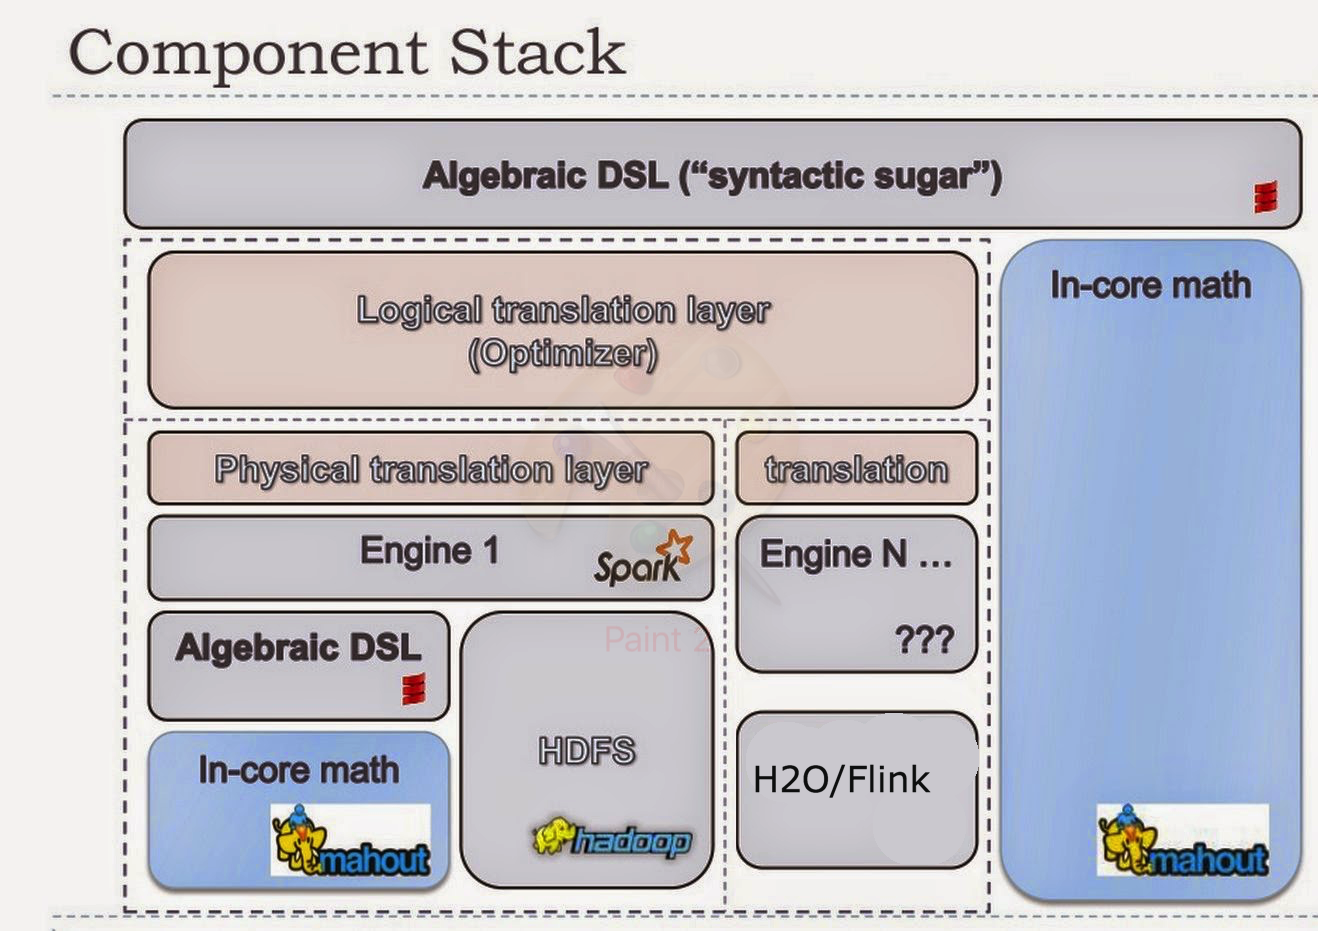
\includegraphics[width=\linewidth]{images/AlgebraOptArchSlide}}
\caption{Mahout Ecosystem. \newline Source: \cite{www-weatheringDays}}
\label{fig:false-color}
\end{figure}
\section{Use Cases}

An use case for recommendation system and a simple linear algebra
operation is provided in this section.

\subsection{Recommendation system with Spark Engine}
A recommendation system is used to recommend most relevant product
that he/she might be interested and boost the sales in online
platforms. Recommendation can be done based on user similarity or item
similarity. In case of user similarity, recommendation is provided
based on idea that users with similar interest would buy similar
products. Similar users are identified, grouped and recommendations
are made based on difference in set of products. Where as item
similarity is based on identifying the products that were bought
together and recommending the products that is not in customer's
basket or purchase history. Recommendation based on item similarity is
very popular in industry as number of product types is way less than
number of customers with regular purchase patterns in large retail
industry.

An illustration of how Mahout can be used with Spark for item based
recommendation is illustrated in figure 2.

\begin{figure}[htbp]
\centering
\fbox{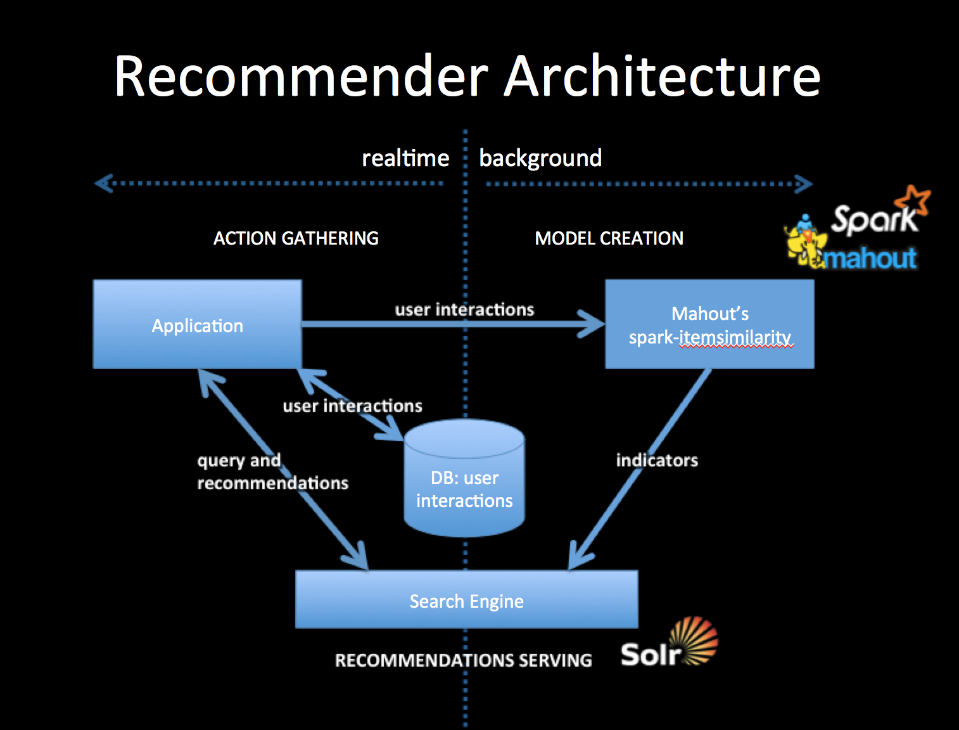
\includegraphics[width=\linewidth]{images/recommender-architecture}}
\caption{Recommender Illustration. \newline Source: \cite{www-recommendations}}
\label{fig:false-color}
\end{figure}

Mahout's mapreduce version of item similarity takes a text file that is
expected to have user and item IDs and provide recommendations based
on content.

\subsection{SPCA}
The equation to compute stochastic principal component analysis is
given in equation 1

\begin{equation}
G=B{B}' - C - {C}' + s_{q} {s_{q}}' {\xi}' \xi\
\label{equation1}
\end{equation}


Mahout code to compute this using Scala DSL is illustrated in
algorithm 1,

\begin{algorithm}
\caption{Mahout DSL to compute SPCA}\label{alg:mahout}
\begin{quote}
\begin{Verbatim}[numbers=left]
val g = bt.t %*% bt - c - c.t + (s_q cross s_q) 
               * (xi dot xi)\
\end{Verbatim}
\end{quote}
\end{algorithm}



This could be used in single or distributed machine in Spark, H2O or
Flink to perform SPCA.

\section{Useful Resources}
Apache Mahout Cookbook\cite{book-mahout} by Piero Giacomelli is a good
introductory book on Mahout. Apache Mahout\: Beyond
MapReduce\cite{book-samsara} by Dmitriy Lyubimov provides an
exhaustive coverage of Mahout Samsara and math operations.

Mahout website\cite{www-mahoutResources} has a compilation of
useful resources like books, tutorials and talks about Mahout and
machine learning.

\section{Conclusion}
Apache Mahout provides an open source environment with scalable
algorithms for machine learning and math operations using DSL. It can
be used with multiple backends like Spark, Scala, Flink and
Hadoop. Same code can be used for single machine and distributed
computing of algorithms in any supported backends.

\section*{Acknowledgements}

This work was done as part of the course "I524: Big Data and
Open Source Software Projects" at Indiana University during
Spring 2017. Thanks to our Professor Gregor von Laszewski
and associate instructors for their help and support during the
course.


% Bibliography

\bibliography{references}


\end{document}